\documentclass{beamer}

\useoutertheme[glossy]{wuerzburg}
\useinnertheme[shadow,outline]{chamfered}
\usecolortheme{shark}
\beamertemplatenavigationsymbolsempty 

\usefonttheme{professionalfonts}
\let\digamma\relax
\usepackage[scale=0.85,stdmathitalics=true,romanfamily=casual]{lucimatx}
\usefonttheme[stillsansseriftext]{serif}


\usepackage{fancyvrb}

%% Fancy syntax coloring via pygments
\usepackage{minted}
\definecolor{bg}{rgb}{0.95,0.95,0.95}
\usemintedstyle{borland}


\newenvironment{Rcode}
{\VerbatimEnvironment
 \begin{minted}[fontsize=\scriptsize,baselinestretch=1]{r}}%
{\end{minted}}

\newenvironment{Pcode}
{\VerbatimEnvironment
 \begin{minted}[fontsize=\scriptsize,baselinestretch=1]{python}}%
{\end{minted}}

\newenvironment{Code}[1]
{\VerbatimEnvironment
 \begin{minted}[fontsize=\scriptsize,baselinestretch=1]{#1}}%
{\end{minted}}


\usepackage{textfit} % commands \scaletoheight{height}{text} and \scaletowidth{width}{text}

\usepackage{tikz}


\newtheorem{Alert}{Alert}
\newtheorem{Highlight}{Highlight}

\newcommand{\Species}[1]{{\rmfamily \itshape #1}}
\newcommand{\Real}{\ensuremath{\mathbb{R}}}
\newcommand{\RealN}{\ensuremath{\mathbb{R}^n}}
\newcommand{\RealP}{\ensuremath{\mathbb{R}^p}}
\newcommand{\Mtx}[1]{\ensuremath{\mathbf{#1}}}
\newcommand{\Inv}[1]{\ensuremath{#1^{-1}}}
\newcommand{\InvMtx}[1]{\ensuremath{\mathbf{#1}^{-1}}}
\newcommand{\Red}[1]{\textcolor{red}{#1}}
\newcommand{\PsInv}[1]{\ensuremath{\mathbf{#1}^{+}}}



\usepackage{amsfonts}
\usepackage{tikz}

\parskip=0.5em

\title{Scientific Computing for Biologists}
\subtitle{Lecture 11: Discriminant Analysis and Classification}

\author{Instructor: Paul M. Magwene}
\date{25 October 2011}


\begin{document}

%===========================================================
\begin{frame}
\titlepage
\end{frame}
%===========================================================


%===========================================================
\begin{frame}
  \frametitle{Outline of Lecture}

\begin{itemize}
    \item Fisher's Discriminant Function    
    \item Canonical Variates Analysis (CVA)
    \begin{itemize}
        \item Geometric and Algebraic View
        \item Similarities and differences between CVA and PCA
        \item Interpretting CVA
        % \item Mahalanobis distance
    \end{itemize}    

\end{itemize}

\end{frame}
%===========================================================


%===========================================================
\begin{frame}
  \frametitle{Overview of Discriminant Analysis}

\begin{block}{Discrimination}
Given an $n \times p$ data matrix, \Mtx{X}, and a grouping of the $n$ specimens into $g$ groups, find the linear combination of the variables, $\Mtx{a}'\Mtx{x}$ that best discriminates between the groups.
\end{block}

\begin{block}{Classification}
Given $g$ groups, define a function that assigns an object with unknown assignment to the `best' group.
\end{block}


\end{frame}
%===========================================================


%===========================================================
\begin{frame}
  \frametitle{Fisher's Discriminant Function}

\begin{itemize}
\item Applies to the two-group case.
\item Solution: find \Mtx{a} that maximizes the ratio of the squared group mean difference to within-group variance:
\end{itemize}

\[
F = \frac{(\Mtx{a}'\bar{\Mtx{x}}_1 - \Mtx{a}'\bar{\Mtx{x}}_2)^2}{\Mtx{a}'\Mtx{W}\Mtx{a}}
\]

where
\begin{itemize}
\item $\bar{\Mtx{x}}_1 = \frac{1}{n_1}\sum_{i=1}^{n_1} \Mtx{x}_{1i}$
\item $\bar{\Mtx{x}}_2 = \frac{1}{n_2}\sum_{i=1}^{n_2} \Mtx{x}_{2i}$
\item $\Mtx{W} = \frac{1}{n_1 + n_2 - 2}\sum_{i=1}^{2}\sum_{j=1}^{n_i}(\Mtx{x}_{ij} - \bar{\Mtx{x}}_i)(\Mtx{x}_{ij} - \bar{\Mtx{x}}_i)'$ (w/in-group pooled covariance matrix)
\item $n_i$ indicates the number of observations in the $i$th group and the $\Mtx{x}_{i1},\ldots,\Mtx{x}_{in_i}$ represent the specific observations (as vectors).
\end{itemize}

% Given an $n \times p$ data matrix, \Mtx{X}, and a grouping of the $n$ specimens into $g$ groups, find the linear coeffients, \Mtx{a}, such that  of the variables, $\Mtx{a}\Mtx{x}_i$ that best discriminates between the groups.
% \end{block}
% 
% Solution: find a that maximizes the ratio of the squared group mean difference to within-group variance:
% 
% 
% 

\end{frame}
%===========================================================

%===========================================================

\begin{frame}
  \frametitle{Geometry of the Two-Group Discriminant Function}
  
\begin{center}
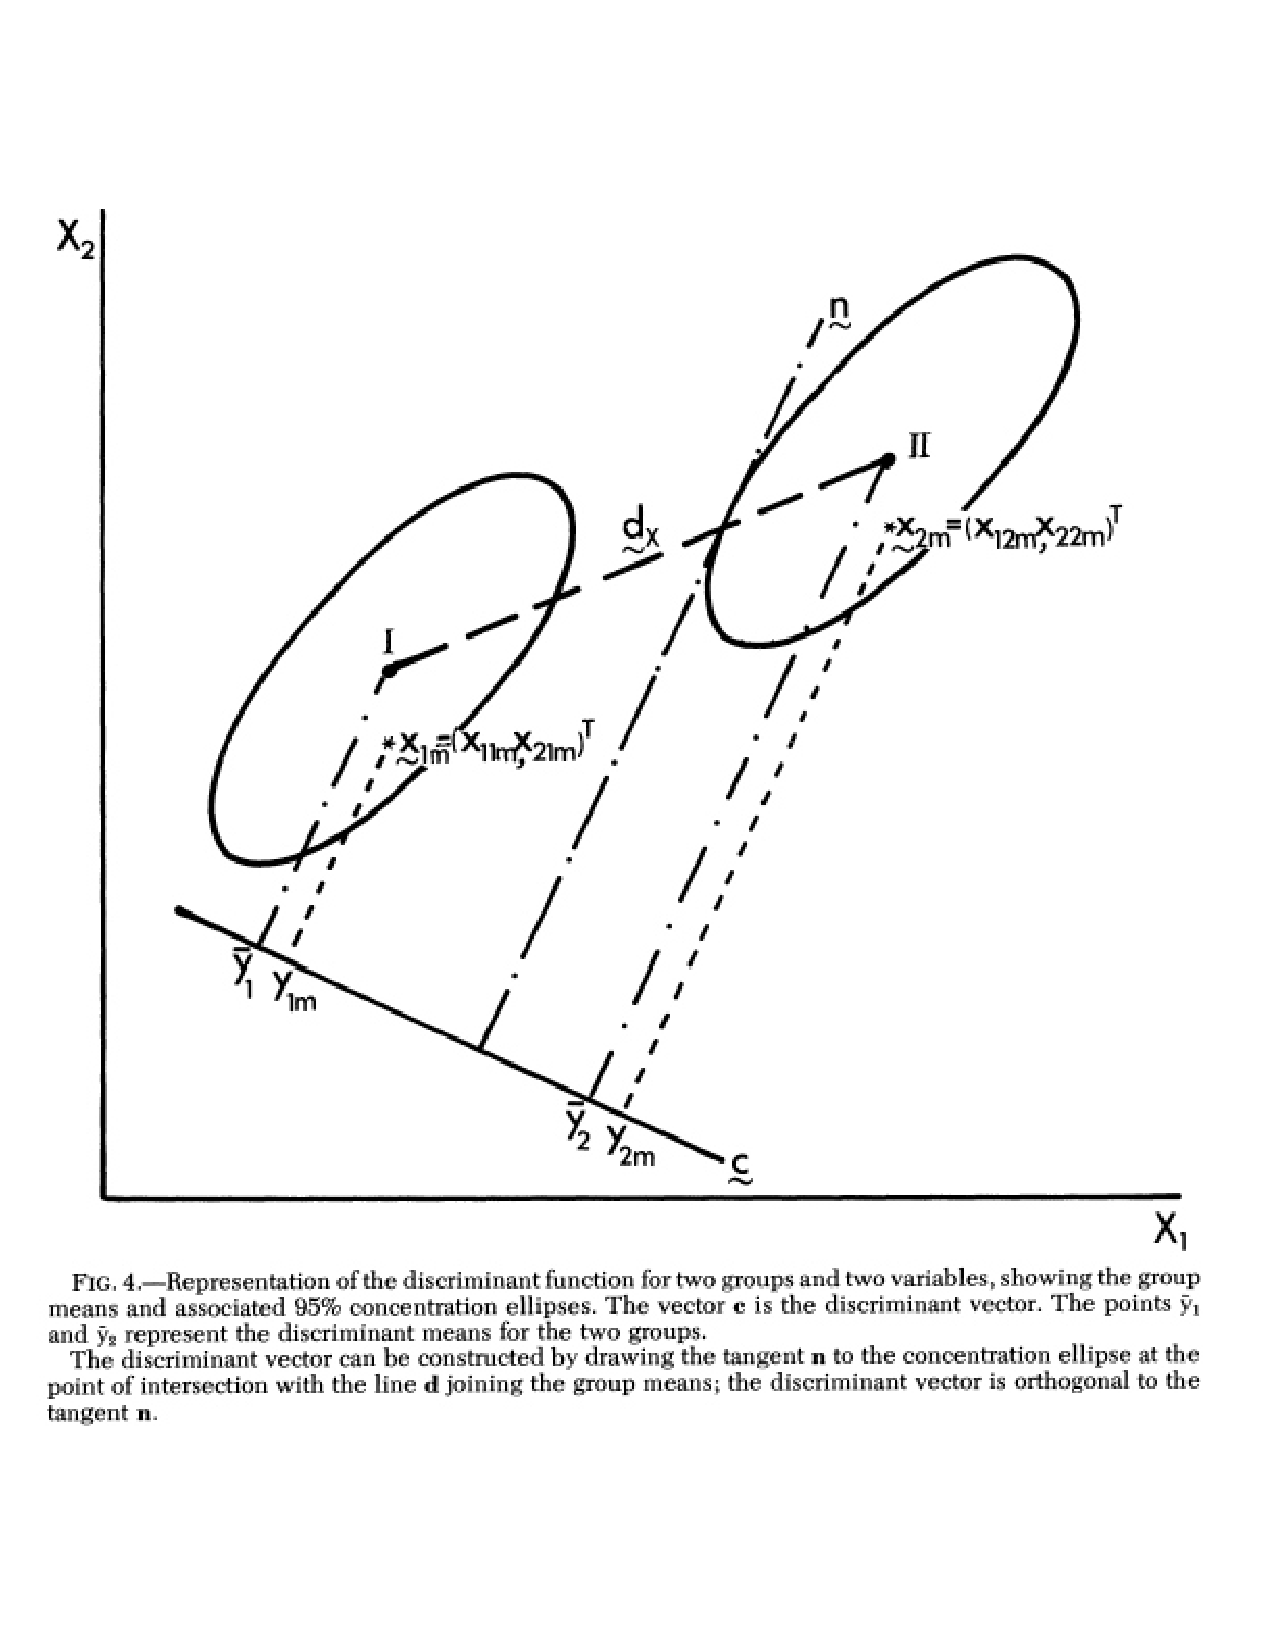
\includegraphics[height=3.1in]{2group}
\end{center}

\end{frame}
%===========================================================

%===========================================================
\begin{frame}
  \frametitle{Fisher's LDF}


\[
F = \frac{(\Mtx{a}'\bar{\Mtx{x}}_1 - \Mtx{a}'\bar{\Mtx{x}}_2)^2}{\Mtx{a}'\Mtx{W}\Mtx{a}}
\]


Maximizing $F$ gives:

\[
\Mtx{a} = c\Mtx{W}^{-1}(\bar{\Mtx{x}}_1 - \bar{\Mtx{x}}_2)
\]

where $c$ is an arbitrary constant (usually taken to be 1).

\end{frame}
%===========================================================


%===========================================================
\begin{frame}
  \frametitle{Fisher's LDF as Classification}

Fisher's solution can also be setup as a classification solution using regression.

\begin{itemize}
\item setup a dummy variable, $y$ that takes the values:
\begin{itemize}
    \item $y_1 = n_2/(n_1 + n_2)$ for observations in group 1
    \item $y_1 = -n_1/(n_1 + n_2)$ for observations in group 2
\end{itemize}
\item Solve the standard multivariate regression, $\Mtx{y} = \Mtx{X}\Mtx{b} + \Mtx{e}$
\item Allocate unknown individual to group 1 if it's predicted $y$ is closer to $y_1$ than to $y_2$, otherwise assign to group 2.

\end{itemize}
\end{frame}
%===========================================================

%===========================================================
\begin{frame}
  \frametitle{What if there are more than two groups?}

The multi-group equivalent of Fisher's LDF is called `Canonical Variate Analysis' (CVA).

\begin{itemize}
\item straight forward extension of Fisher's solution
\item Find \Mtx{a} that maximizes the ratio of between-group to within-group variance:

\[
F = \frac{\Mtx{a}'\Mtx{B}\Mtx{a}}{\Mtx{a}'\Mtx{W}\Mtx{a}}
\]

\item \Mtx{W} is within-group matrix (as defined previously)
\item \Mtx{B} is the between-group covariance matrix
\begin{itemize}
    \item $\Mtx{B}_w = \frac{1}{g-1}\sum_{i=1}^{g} n_i(\Mtx{x}_i - \bar{\Mtx{x}})(\Mtx{x}_i - \bar{\Mtx{x}})'$ where $n_i$ is the sample size in group $i$ (weighted version)
    \item  $\Mtx{B}_u = \frac{1}{g-1}\sum_{i=1}^{g} (\Mtx{x}_i - \bar{\Mtx{x}})(\Mtx{x}_i - \bar{\Mtx{x}})'$ (unweighted version)
\end{itemize}

\end{itemize}

\end{frame}
%===========================================================

%===========================================================
\begin{frame}
  \frametitle{Geometry of CVA}
  
\begin{center}
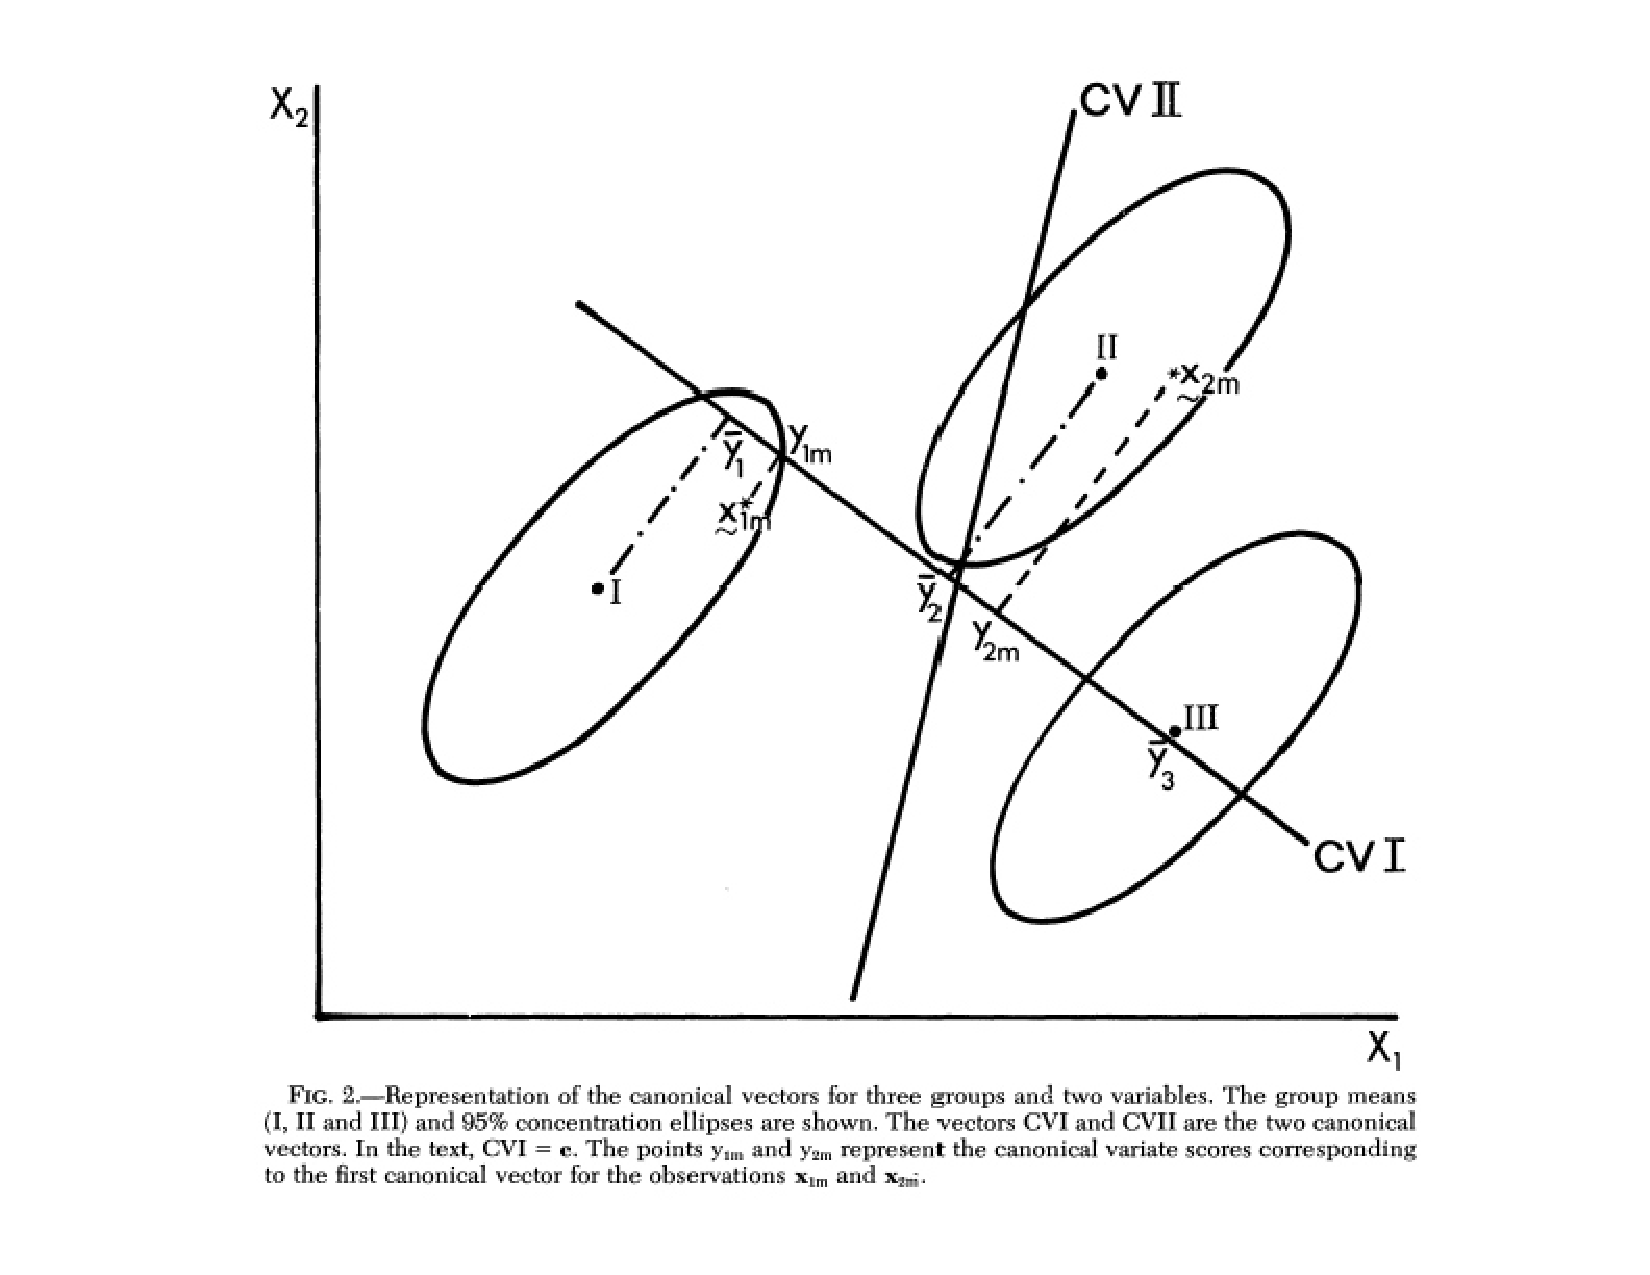
\includegraphics[height=3.1in]{3group}
\end{center}

\end{frame}
%===========================================================


%===========================================================
\begin{frame}
  \frametitle{CVA Solution}

Maximizing $F$ leads to the following:
\[
(\Mtx{B} - l\Mtx{W})\Mtx{a} = \Mtx{0}
\]

\begin{itemize}
\item $l$ is an eigenvalue of $\Mtx{W}^{-1}\Mtx{B}$
\item $\Mtx{a}$ is an eigenvector of $\Mtx{W}^{-1}\Mtx{B}$
\end{itemize}

There will be $s=\min(p, g-1)$ non-zero eigenvalues.
\medskip

Organize the eigenvectors, $\Mtx{a}_i$, as columns of a $p \times s $ matrix \Mtx{A}. 
\begin{itemize}
\item The \textbf{\emph{canonical variates}} are given by $\Mtx{y} = \Mtx{A}'\Mtx{x}$
\item The mean of the $i$th group in the canonical variates space is given by $\bar{\Mtx{y}}_i = \Mtx{A}'\bar{\Mtx{x}}_i$
\end{itemize}

\end{frame}
%===========================================================

%===========================================================
\begin{frame}
  \frametitle{CVA as a two-stage rotation I}
  
\begin{center}
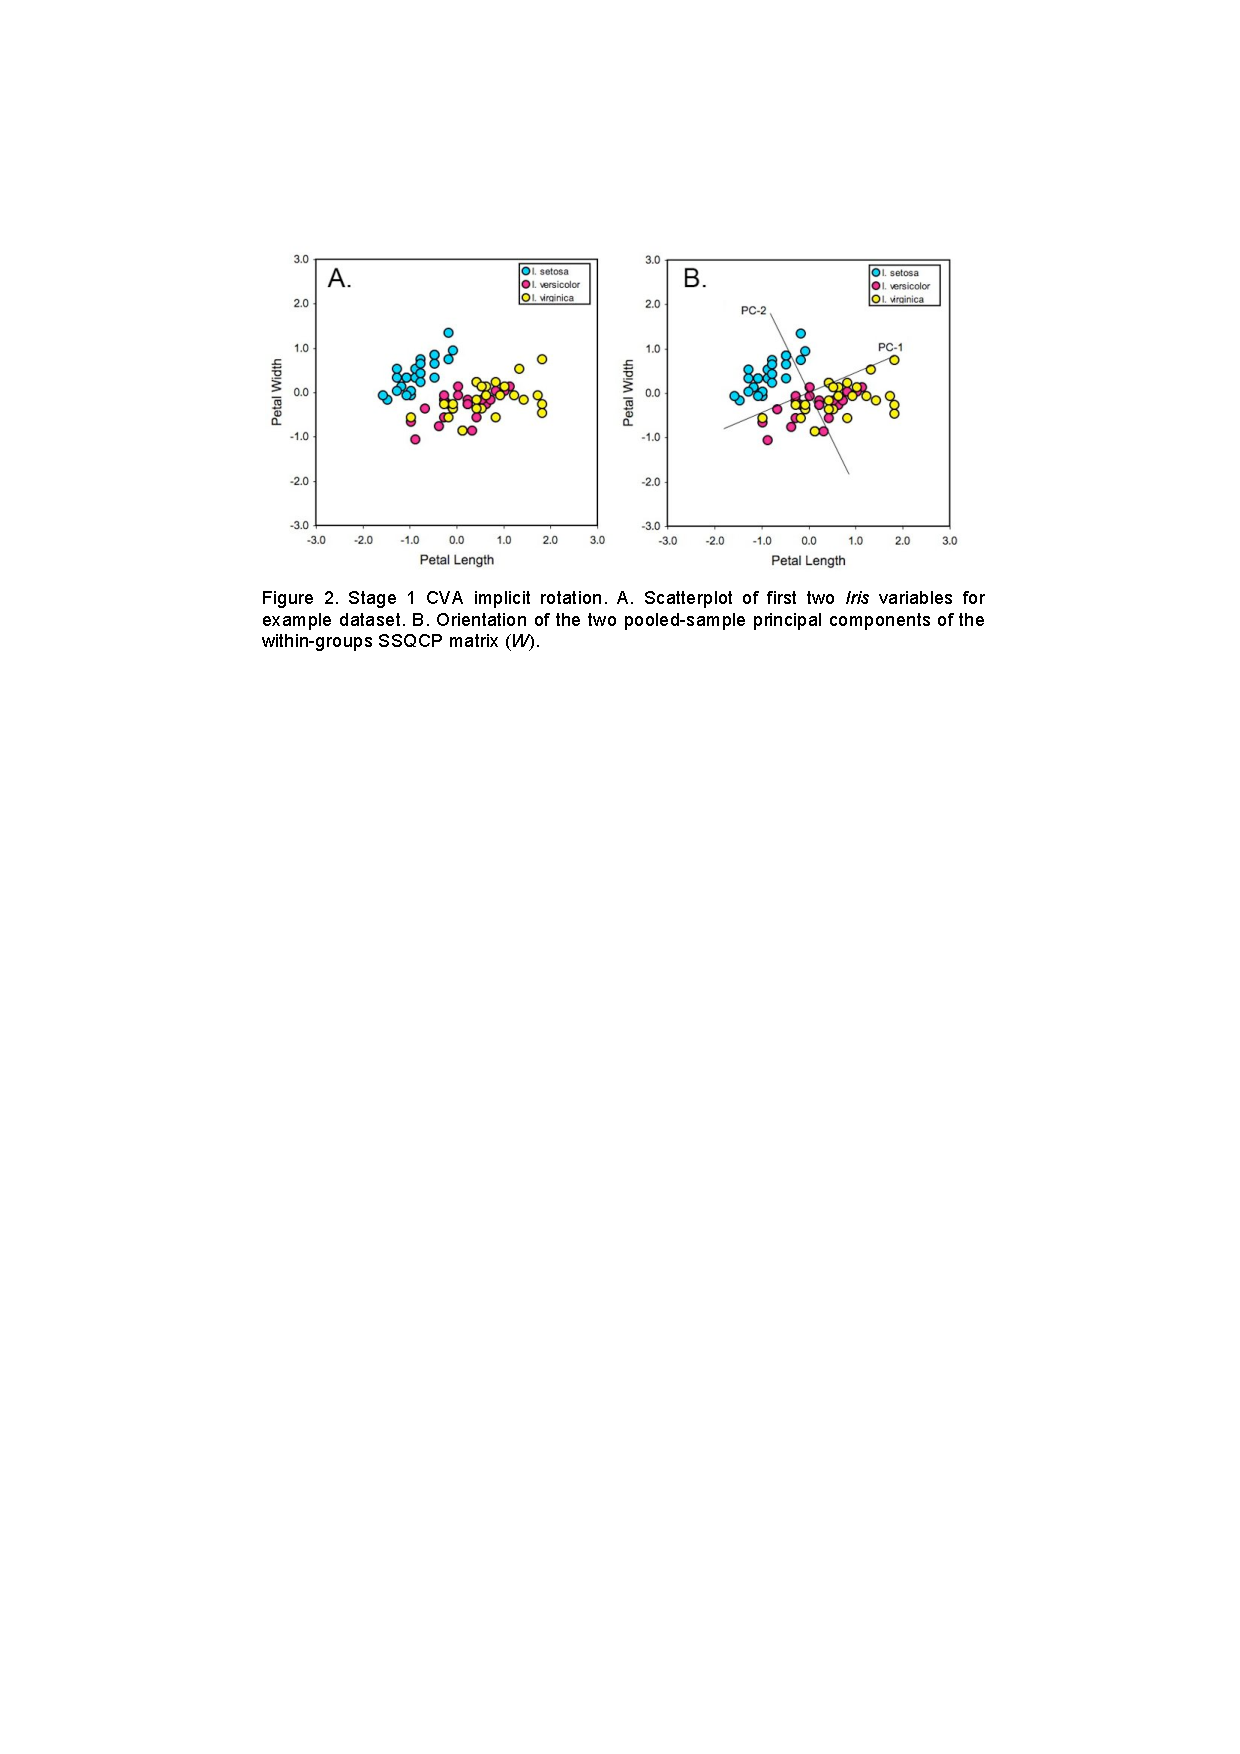
\includegraphics[width=\textwidth]{cva-as-rot1}
\end{center}

\hfill {\scriptsize \textit{From MacLeod 2010, PalaeoMath newsletter}}

\end{frame}
%===========================================================

%===========================================================
\begin{frame}
  \frametitle{CVA as a two-stage rotation II}
  
\begin{center}
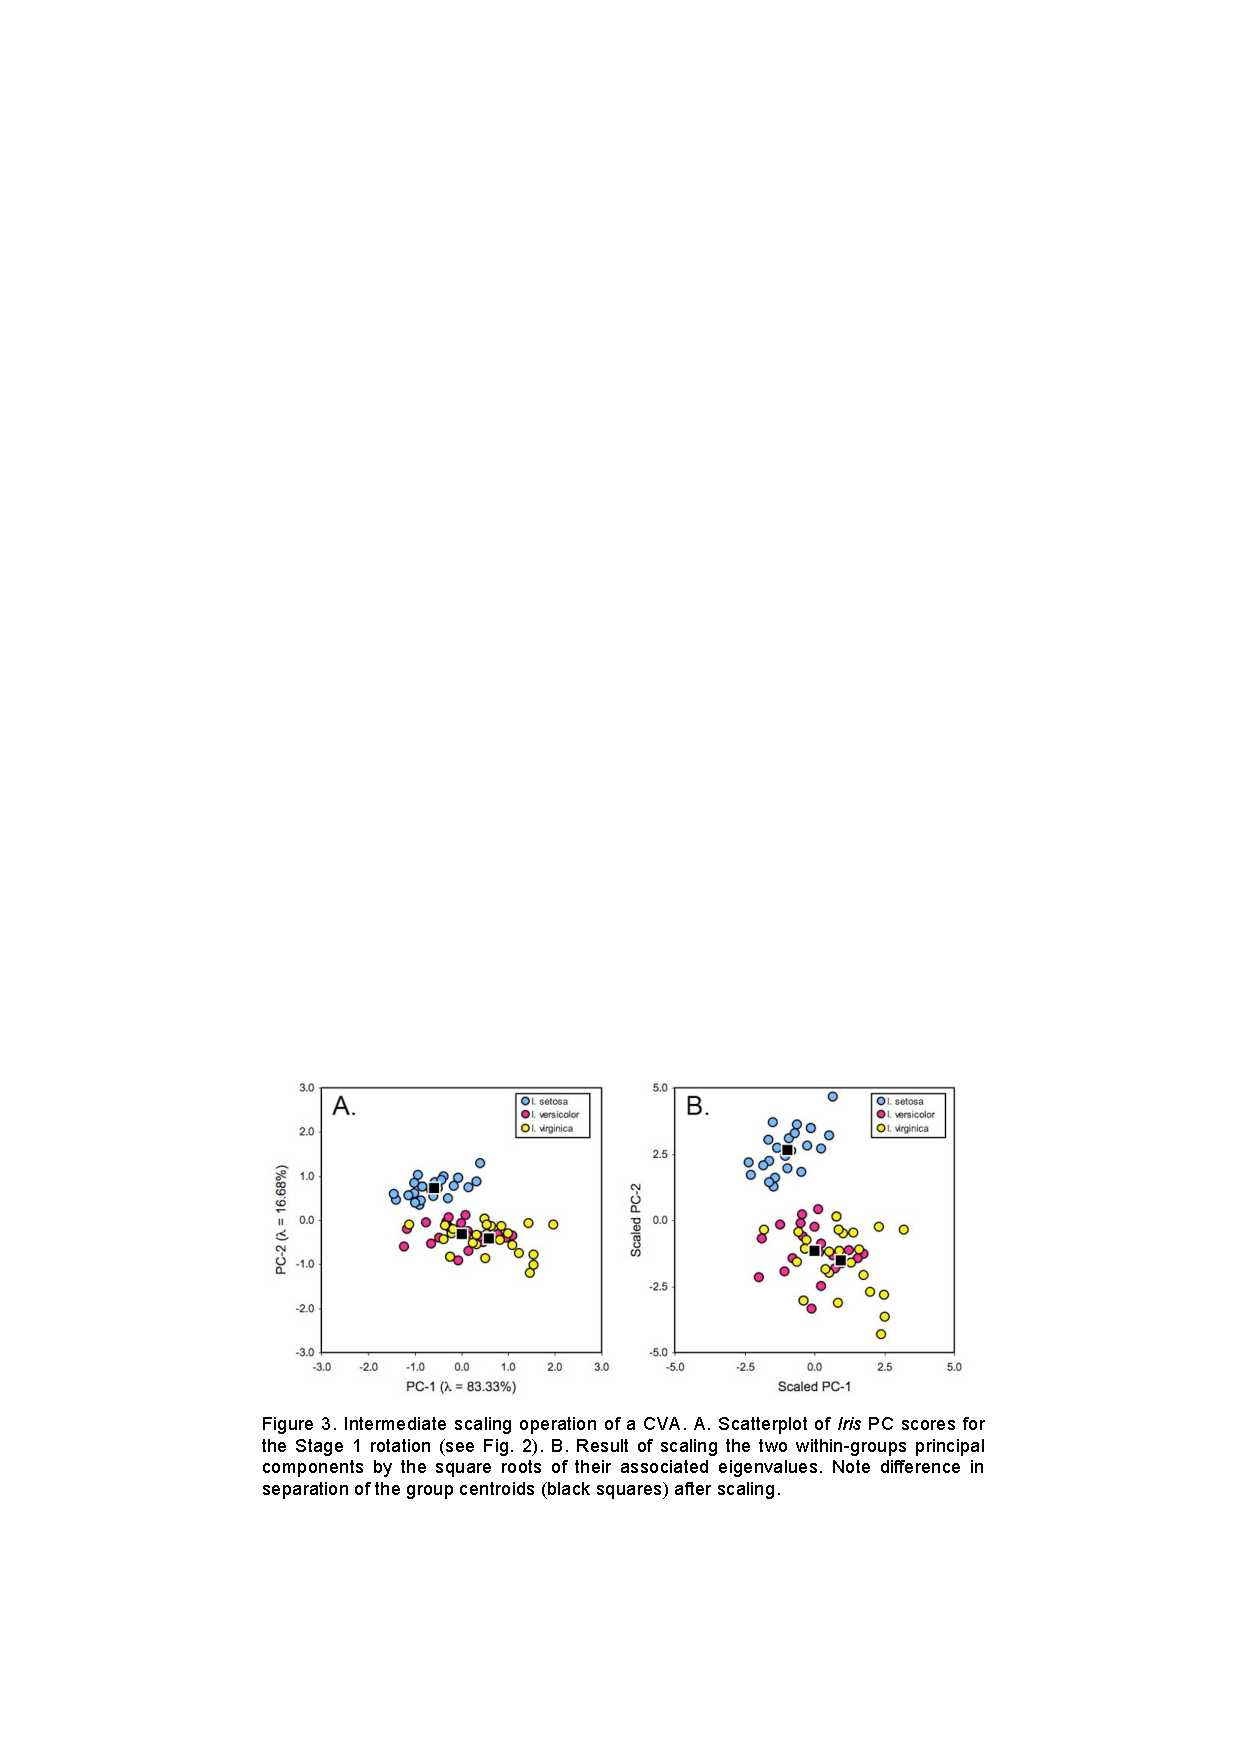
\includegraphics[width=0.9\textwidth]{cva-as-rot2}
\end{center}

\hfill {\scriptsize \textit{From MacLeod 2010, PalaeoMath newsletter}}


\end{frame}
%===========================================================

%===========================================================
\begin{frame}
  \frametitle{CVA as a two-stage rotation III}
  
\begin{center}
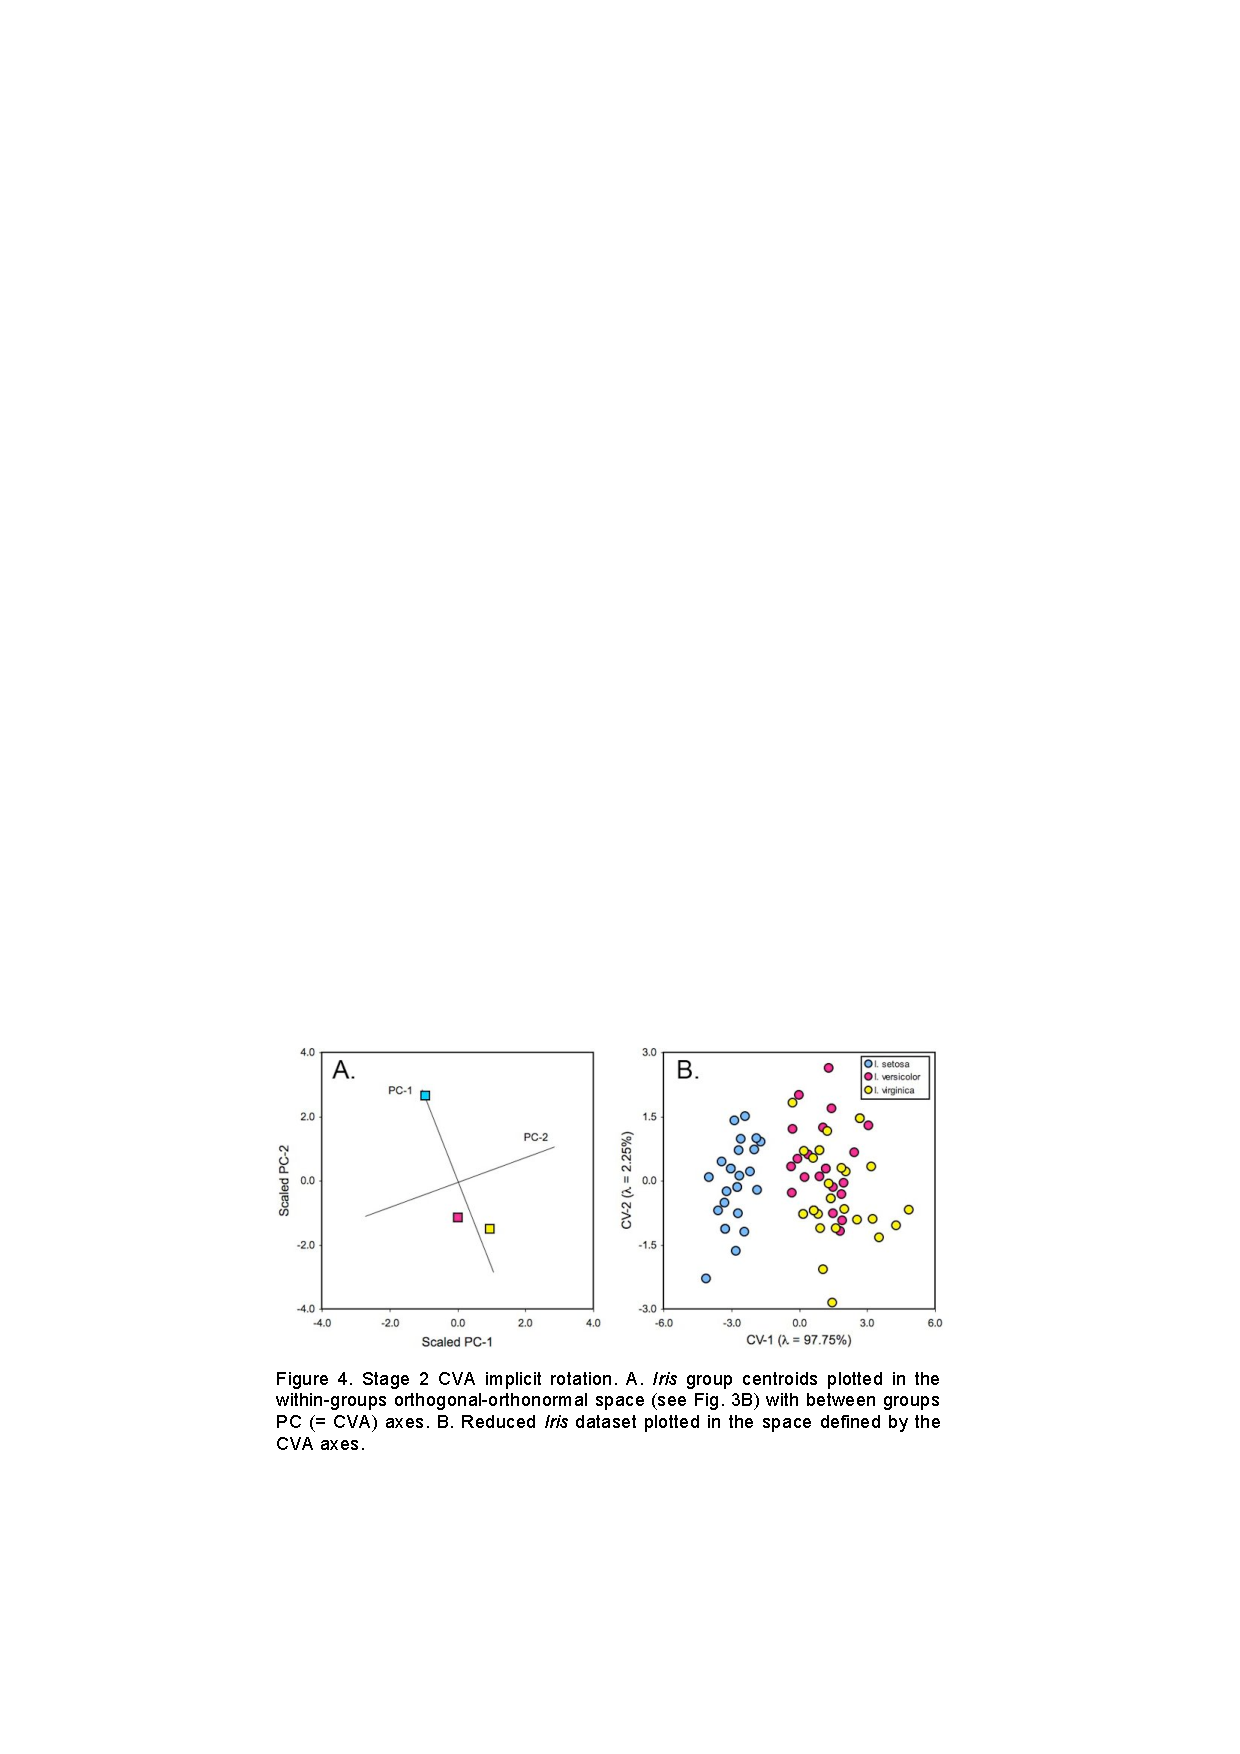
\includegraphics[width=0.9\textwidth]{cva-as-rot3}
\end{center}

\hfill {\scriptsize \textit{From MacLeod 2010, PalaeoMath newsletter}}


\end{frame}
%===========================================================

%===========================================================
\begin{frame}
  \frametitle{CVA as a two-stage rotation IV}
  
\begin{center}
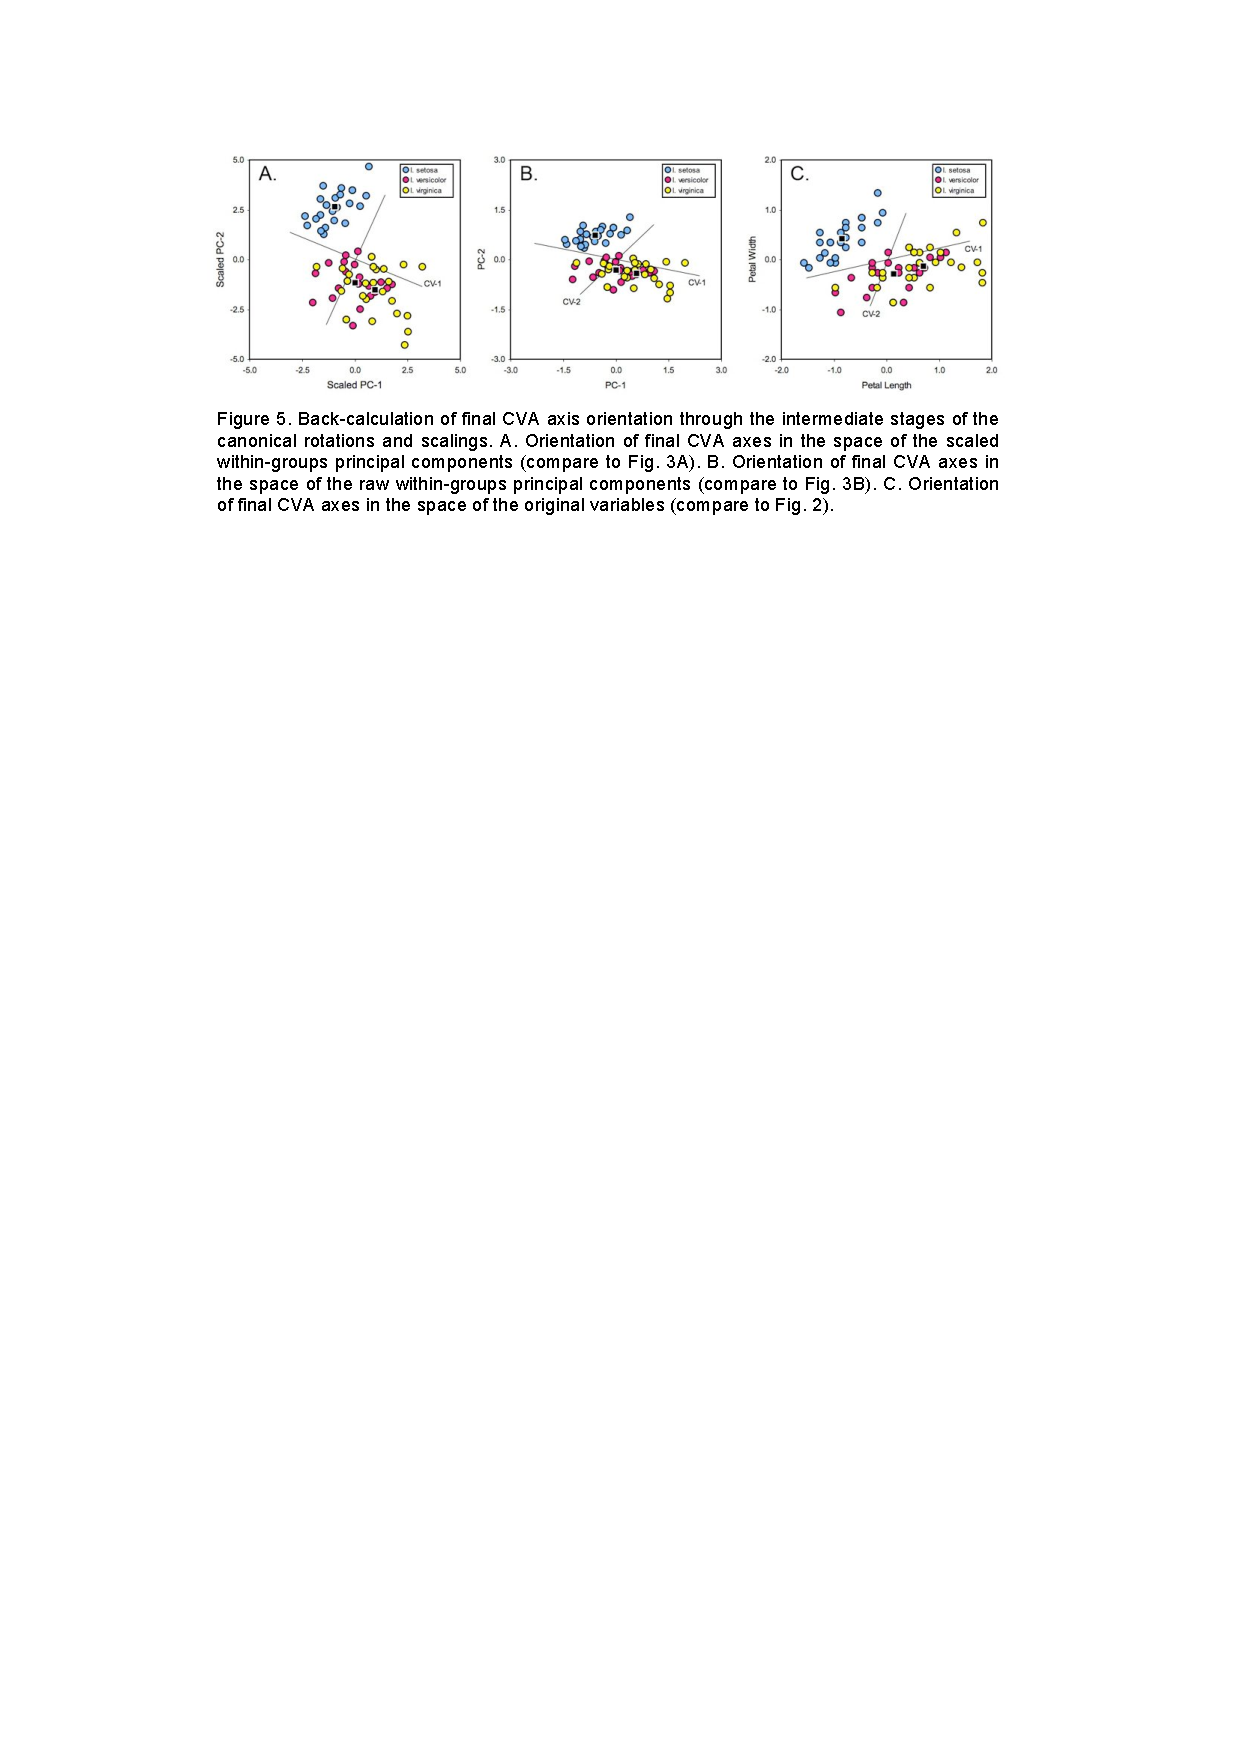
\includegraphics[width=\textwidth]{cva-as-rot4}
\end{center}

\hfill {\scriptsize \textit{From MacLeod 2010, PalaeoMath newsletter}}

\end{frame}
%===========================================================


%===========================================================
\begin{frame}
  \frametitle{Similarities and Differences between CVA and PCA}
  
PCA:
\begin{itemize}
\item Uncorrelated over the whole sample
\item orthogonal transformation from the original variates, \Mtx{x}, to the new variates \Mtx{y}. PC axes at right angles to each other in the space of the original variables.
\end{itemize}

CVA:
\begin{itemize}
\item Canonical variates are uncorrelated both \emph{within} and \emph{between} groups
\item Canonical variates have equal variance \emph{within} groups, but in decreasing order \emph{between} groups
\item non-orthogonal transformation, CV axes \emph{not} at right angle to each other in the original frame of reference.
\end{itemize}
\end{frame}

%===========================================================
%@nonl
%@-node:pmagwene.20061107103153:Similarities/Differences w/PCA
%@+node:pmagwene.20061107110604:Illustration of PCA vs CVA


%===========================================================
\begin{frame}
  \frametitle{PCA vs CVA: A Motivating Example}

\begin{center}
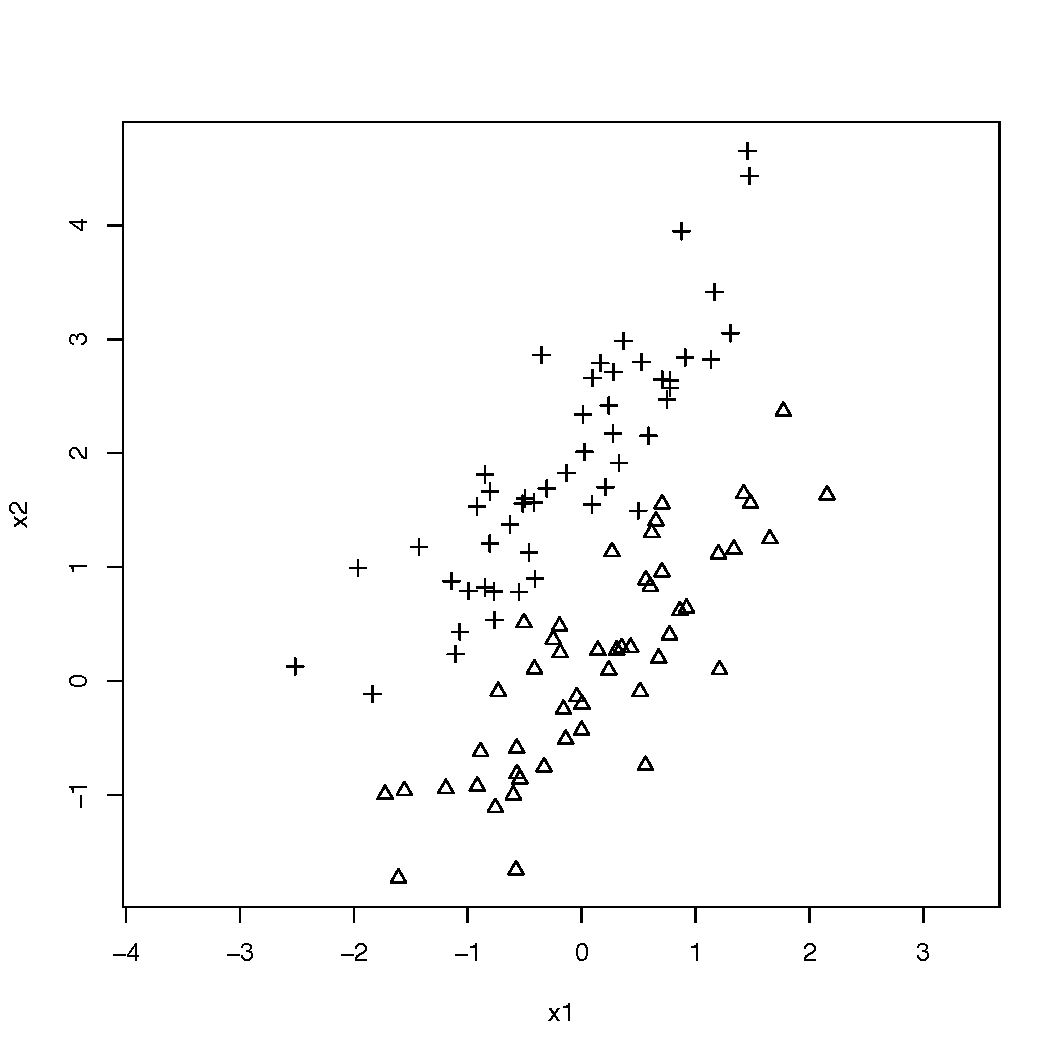
\includegraphics[height=2.5in]{simple2group}

What is the direction of PC1? What is the direction of CVI?
\end{center}

\end{frame}
%===========================================================

% %===========================================================
% \begin{frame}
%   \frametitle{The different components of interest}
% 
% \begin{center}
% 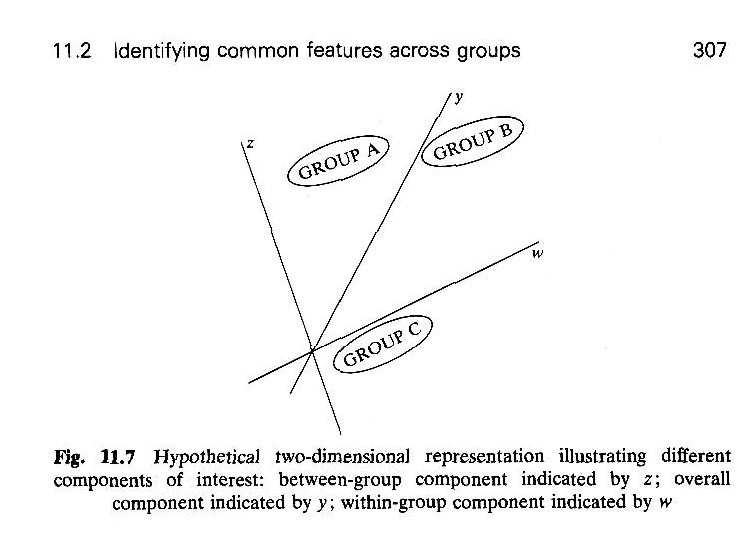
\includegraphics[height=3in]{krz-components}
% \end{center}
% 
% \end{frame}
% %===========================================================


%===========================================================
\begin{frame}
  \frametitle{PCA vs. CVA: Anderson's Iris Data}

\begin{columns}

\begin{column}{0.5\textwidth}
\begin{center}
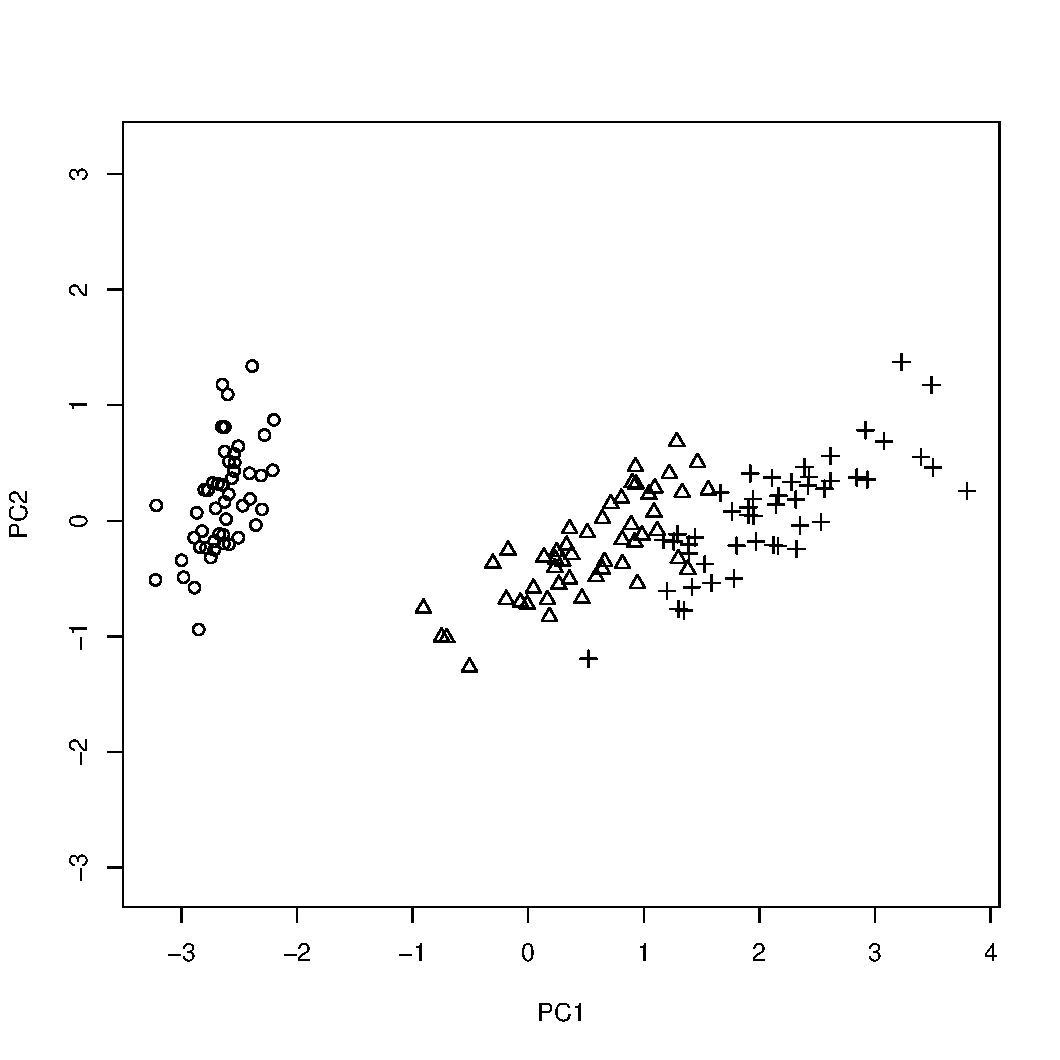
\includegraphics[width=\textwidth]{iris-PCA}
\end{center}
\end{column}

\begin{column}{0.5\textwidth}
\begin{center}
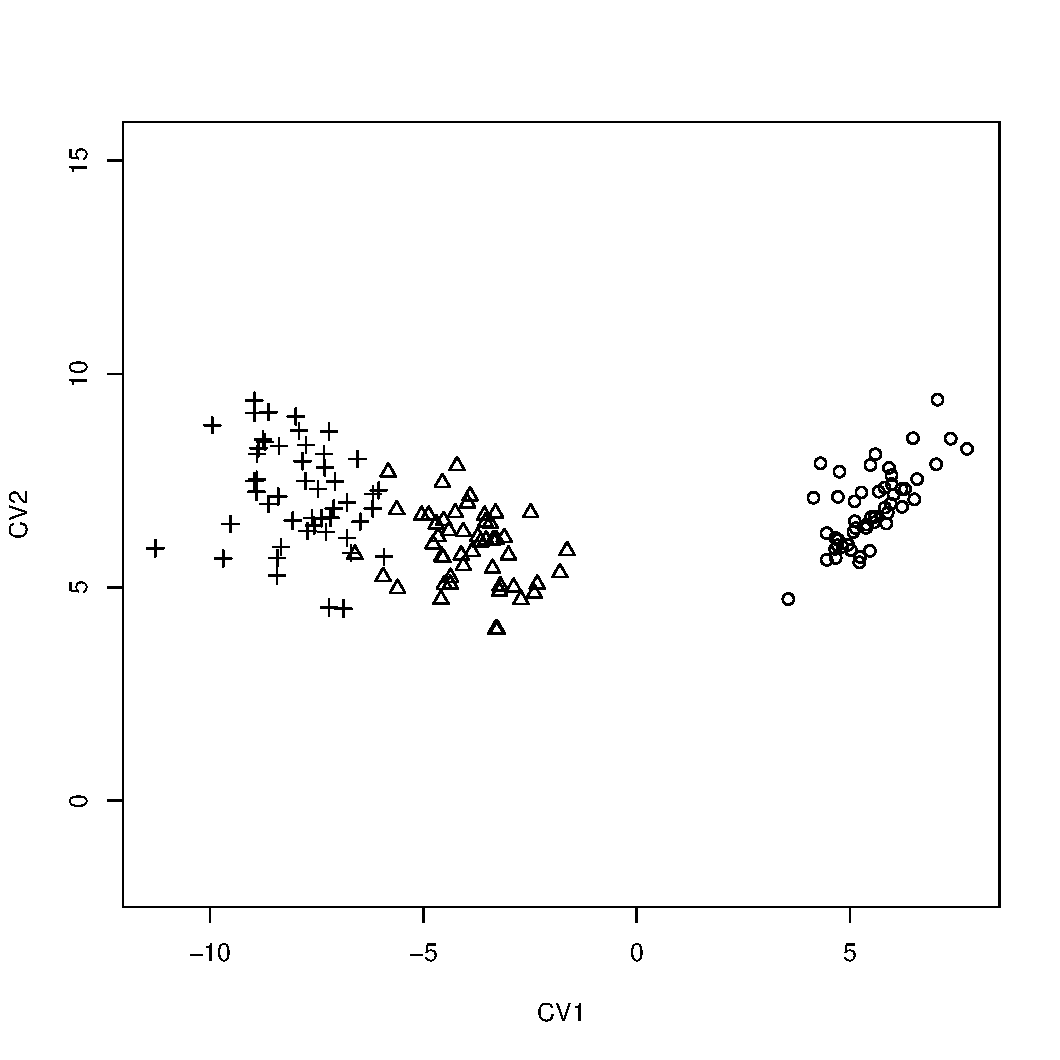
\includegraphics[width=\textwidth]{iris-CVA}
\end{center}
\end{column}

\end{columns}
\end{frame}
%===========================================================

% %===========================================================
% \begin{frame}
%   \frametitle{Mahalanobis Distance I}
%  
% \begin{block}{Question} 
% If canonical variates are not orthogonal, what justifies plotting them as so?
% \end{block}
% 
% \begin{block}{Answer}
% A consideration of multivariate distance is the justification for orthogonal representation of CVs.
% \end{block}
% 
% 
% \end{frame}
% %===========================================================
% 
% %===========================================================
% \begin{frame}
%   \frametitle{Mahalanobis Distance II}
%  
% Consider:
% \begin{itemize}
% \item if all variates have equal variances and are uncorrelated w/in groups than Euclidean distance between group means is an accurate representation of (statistical) dissimilarity
% \item However, if some variables have very large variance or pairs of variables are highly correlated than Euclidean distance between group means isn't a good representation of the `true' dissimilarity in terms of variational trends
% \end{itemize}
% 
% see illustration on board.
% 
% \end{frame}
% %===========================================================
% 
% %===========================================================
% \begin{frame}
%   \frametitle{Mahalanobis Distance III}
% 
% A dissimilarity measure that takes into account patterns of variance/covariance is called `Mahalanobis Distance'.
% 
% The Mahalanobis distance between the $i$th and $j$th group means is given by:
% \[
% D^2 = (\bar{\Mtx{x}}_i - \bar{\Mtx{x}}_j)' \Mtx{W}^{-1} (\bar{\Mtx{x}}_i - \bar{\Mtx{x}}_j)
% \]
% 
% It turns out that by constructing orthogonal axes from the canonical variates than Euclidean distance in the canonical variate space corresponds  (approximately) to Mahalanobis distance in the original variate space.
% 
% \emph{Sidenote} -- The distance between the individual point $\Mtx{x}_i$ and the mean of a $\bar{\Mtx{x}}$ of a single sample is given by $d^2 = (\Mtx{x}_i - \bar{\Mtx{x}})' S^{-1} (\Mtx{x}_i - \bar{\Mtx{x}})$ where \Mtx{S} is the covariance matrix.
% 
% \end{frame}
% %===========================================================

%===========================================================
\begin{frame}
  \frametitle{Are any of the groups significantly different in the canonical variate space?}

To test:
\begin{itemize}
\item $H_0: \mu_1 = \mu_2 = \ldots = \mu_3$
\item $H_1$: at least one $\mu_i$ differs from the rest
\end{itemize}

A couple of approaches:
\begin{itemize}
\item  Compare the largest eigenvalue, $l_1$, of $\Mtx{W}^{-1}\Mtx{B}$ to critical values in a F-table. $H_0$ is rejected for large values ($>1$).
\item Likelihood approach: 
\begin{itemize}
\item Wilks' lambda, $\Lambda = |\Mtx{W}|/|\Mtx{B} + \Mtx{W}| = \prod_{i=1}^{p} (1 + l_i)^{-1}$
\item there is an approximation that has a $\chi^2$ distribution.
\end{itemize}
\end{itemize}

Both boil down to a consideration of eigenvalues of $\Mtx{W}^{-1}\Mtx{B}$.

\end{frame}
%===========================================================


%===========================================================
\begin{frame}
  \frametitle{Which groups are different? Where does an unassigned observation belong?}
  
Within groups the canonical variates are: 
\begin{itemize}
\item uncorrelated
\item have unit variance
\end{itemize}

If we assume multivariate normality of the data then we can exploit this to draw confidence intervals around the group means in the canonical variate space.
\smallskip

A 100(1-$\alpha$) percent confidence region for the true mean $\Mtx{v}_i$ is given by:
\begin{itemize}
\item hypersphere centered at $\bar{\Mtx{y}}_i$
\item with radius ($\chi^{2}_{\alpha,r}/n_i)^{1/2}$ where $r$ is the number of canonical variate dimensions considered
\end{itemize}

\end{frame}
%===========================================================


%===========================================================
\begin{frame}
  \frametitle{Illustration of group means and tolerance regions}

\begin{center}
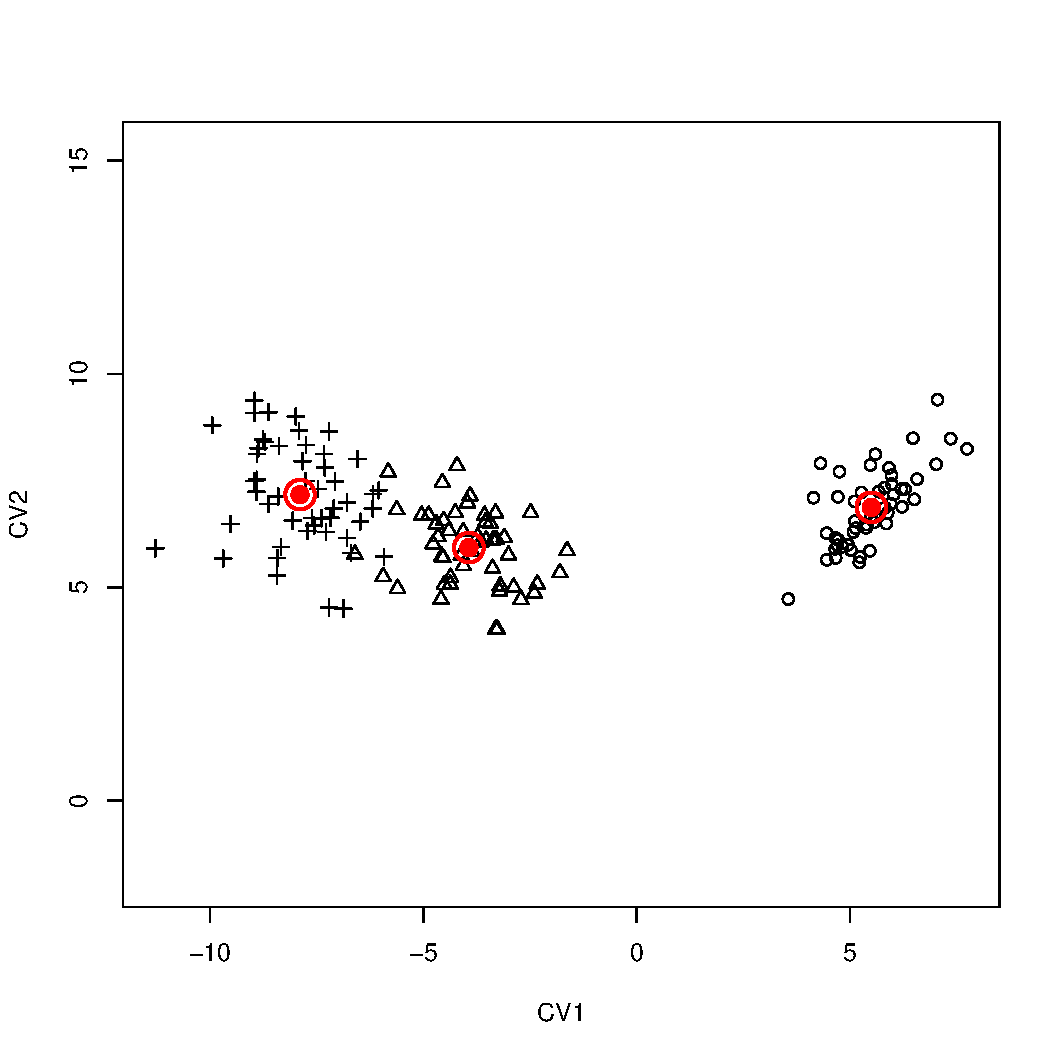
\includegraphics[height=3.1in]{iris-CVA-meantol}
\end{center}

\end{frame}
%===========================================================


%===========================================================
\begin{frame}
  \frametitle{Which variables are most important in CVA?}

\begin{block}{Question}
Which variables are most 'important' in distinguishing between the groups?
\end{block}

Consider the coefficients $\Mtx{a}_i$
\begin{itemize}
\item large coefficients may be due to \emph{either} large between-group variability \emph{or} small within-group variability of the corresponding variable
\item for interpretation it's better to consider modified coefficient, $\Mtx{a}_{i}^{*} = (a_{i1}^{*},\ldots,a_{ip}^{*})$ where the $a_{ij}^{*}$ are given by $a_{ij}^{*} = a_{ij}\sqrt{w_{jj}}$ [$w_{jj}$ are the diagonal elements of \Mtx{W}].
\end{itemize}

\end{frame}
%===========================================================


% %===========================================================
% \begin{frame}
%   \frametitle{CVA as a two-step PCA}
% 
% \begin{center}
% 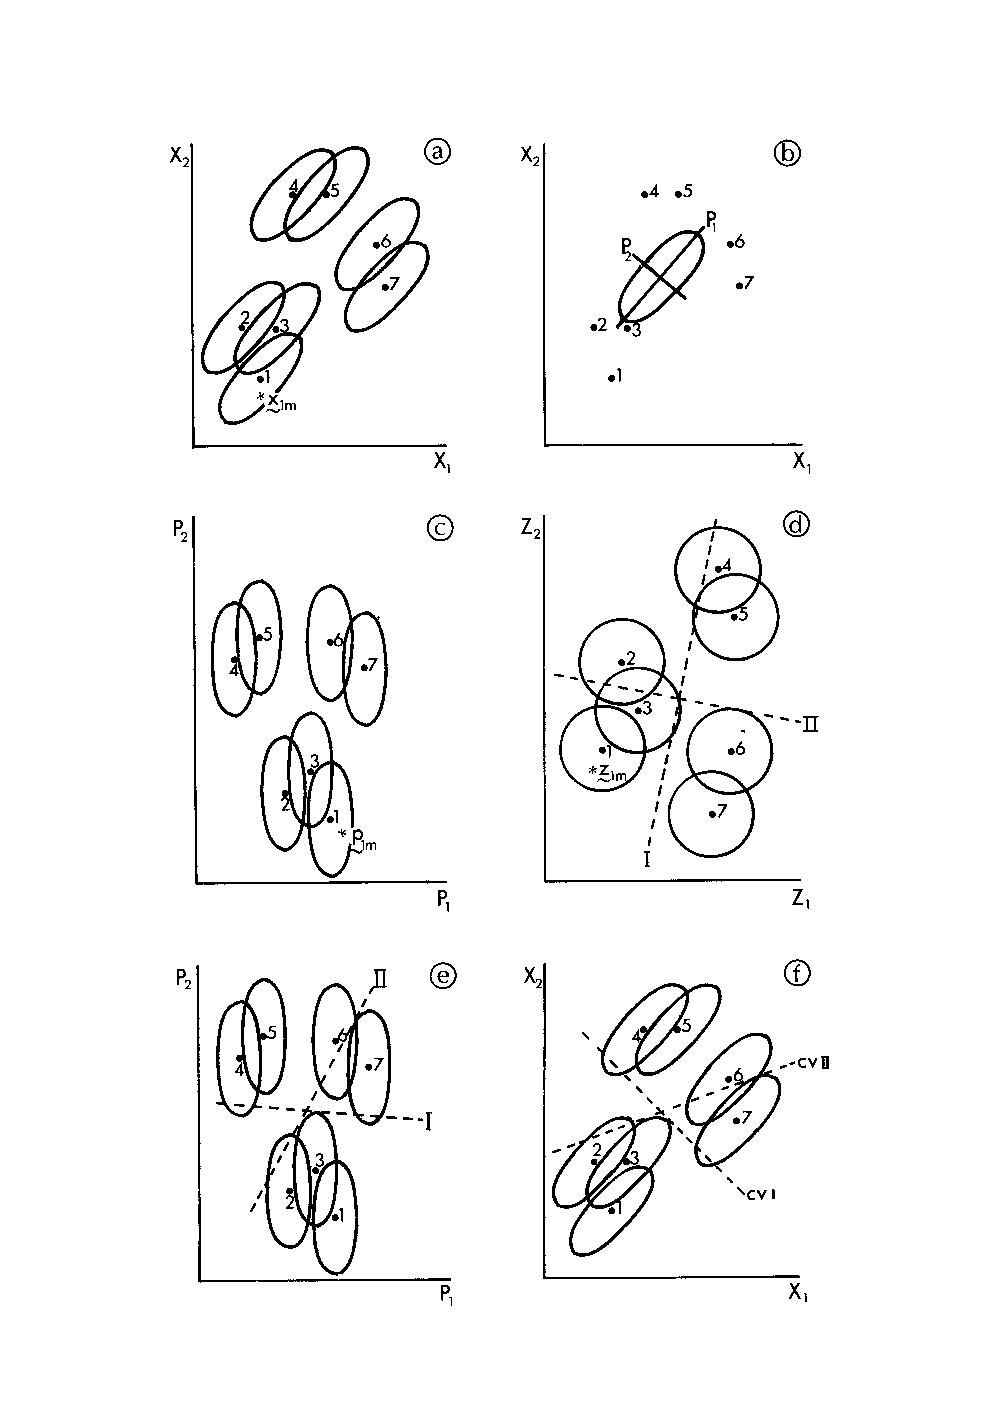
\includegraphics[height=3.2in]{two-step-cva}
% \end{center}
% 
% \end{frame}
% %===========================================================


\end{document}
